\chapter{Resultados e Discussão}\label{cap:resultados}

\section{Sequenciamento e controle de qualidade das leituras}
Após o sequenciamento das amostras, foram obtidas 7.8 milhões de leituras de tamanho médio de 
223 pares de base para a amostra ACT016 e 7.4 milhões de leituras com tamanho médio de 222 pares de base
para a amostra FIR\_094. Após a filtrar as leituras utilizando a ferramenta Trimmomatic, retivemos
6.2 milhões de leituras com tamanho médio 113 pares de base \(perda 21,5\%\) para ACT016 e 6.1 milhões
de leituras com tamanho médio 145 pares de base\(perda de 18,5\%\).

Baseando-se num tamanho de genoma variável de 3 a 10 milhões de bases para \textit{Rhodococcus}, podemos
determinar a cobertura real estimada pela fórmula $C= (L\cdot N)/G $ sendo $C$ a cobertura, $L$ o comprimento
médio das reads e $G$ o tamanho do genoma. A partir disso, obtivemos que a cobertura para a amostra ACT016 Após
filtrar as leituras está entre $70$ e $233,53$ vezes. 
Para a amostra FIR\_094, consideramos o tamanho do genoma de referência de \textit{Brevibacillus Brevis}$($NZ\_LR134338$)$ 
de 6.2 milhões de bases e estimamos a cobertura em aproximadamente $142,66$ vezes.

As qualidades médias das sequências pode ser observada a partir dos gráficos a seguir gerados pela ferramenta FASTQC:

\begin{figure}[H]
	\caption{Gráficos representando a qualidade média das leituras da amostra ACT016 na escala PHRED}
	\centering
	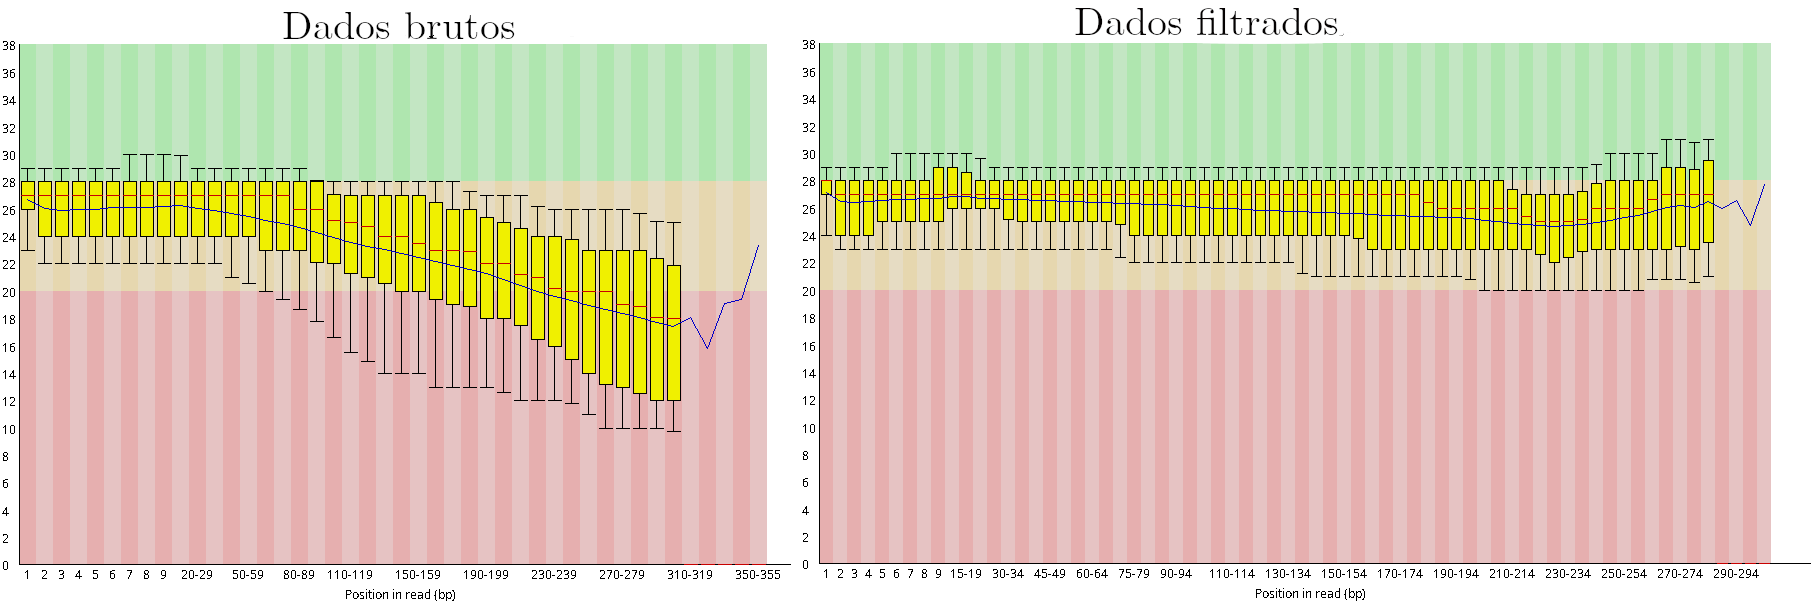
\includegraphics[width=0.8\linewidth]{imagens/read\_qc/002merged.png} \\
	\centering
	\legend{Box plot representando a distribuição da variação média de qualidade das leituras (eixo Y) em relação a posição
	da base na leitura $($eixo X$)$, a linha azul representa a média. As cores verde, amarelo e vermelho representam respectivamente: qualidade excelente $($\textgreater$)$,
	 boa $($\textless 27; \textgreater =20$)$ e ruim$($\textless 20$)$.}
\end{figure}

\vspace{\floatsep}

\begin{figure}[H]
	\caption{Gráficos representando a qualidade média das leituras da amostra FIR\_094 na escala PHRED}
	\centering
	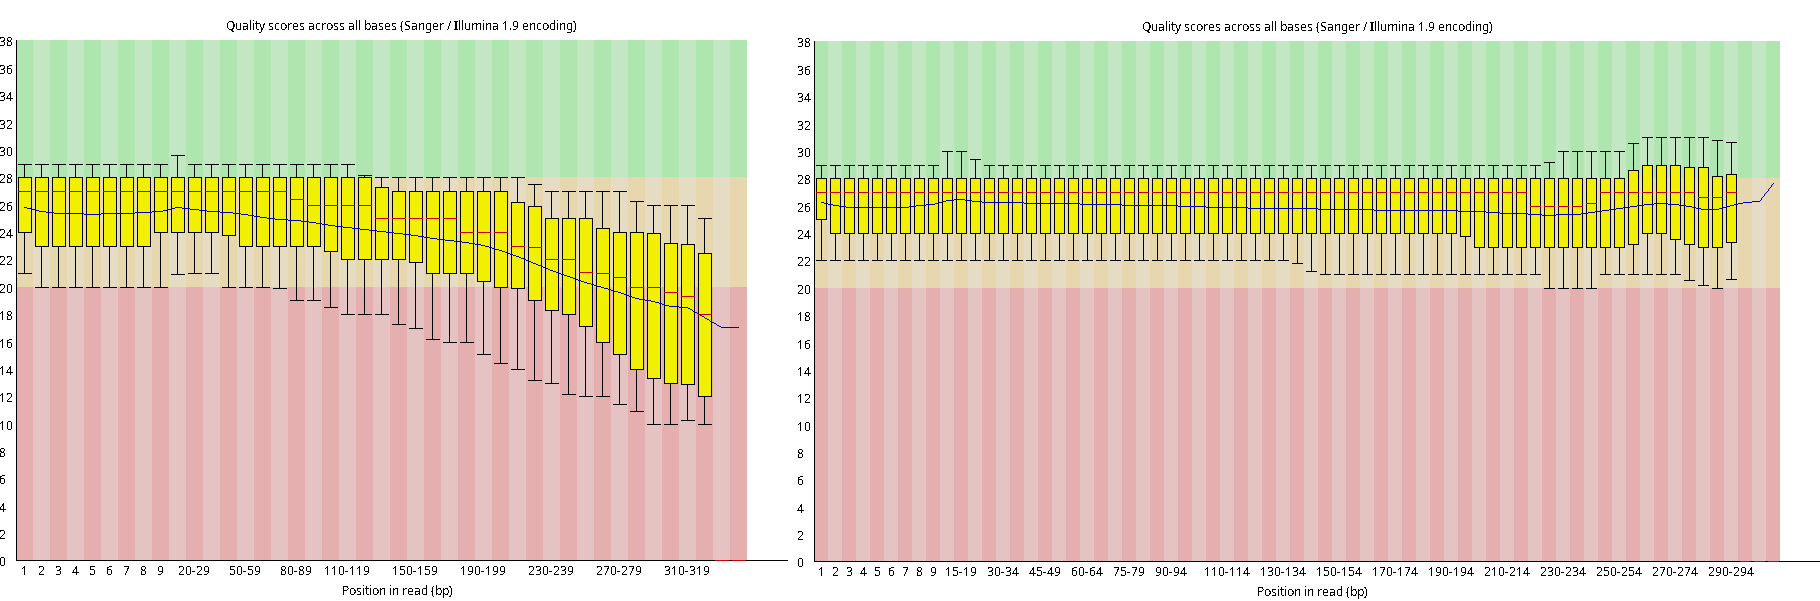
\includegraphics[width=0.8\linewidth]{imagens/read\_qc/004merged.png} \\
	\centering
    \begin{small}\textbf{Fonte: autoria prória}\end{small}
\end{figure}
\vspace{\floatsep}

A partir desses gráficos podemos observar a perda de qualidade no final das leituras, um tipo de limitação
técnica comum ao utilizar sequenciadores da plataforma \textit{Illumina}, porém o término em baixa qualidade
pode ser removido após a filtração, tendo uma qualidade média ao longo da sequência próximo de PHRED 26 e
removendo sequências abaixo de PHRED 20 $($ que representa probabilidade de erro maior que 1 em 100$)$.


\section{Montagem das \textit{contigs}}
\begin{table}[htb]
	\IBGEtab{%
	  \caption{Relatório do software QUAST para as montagens da amostra 016}%
	  \label{tabela-quast016}
	}{%
	\begin{tabular}{lllll}
		
		\toprule
		\textbf{Estatística} & \multicolumn{3}{l}{Nome das montagens}                                                                                                                       &                                 \\
		\cmidrule{2-5}
		                         & \textbf{bactopia+skesa} & \textbf{bactopia+spades} & \textbf{manual mais kmers} & \textbf{manual+spadess}\\
		\midrule
		Número de contigs                            & 2893                                   & 2859                                    & 267                               & 211                                         \\
		Número de contigs (\textgreater{}= 0 bp)     & 2893                                   & 2859                                    & 373                               & 314                                        \\
		Número de contigs (\textgreater{}= 1000 bp)  & 2088                                   & 2069                                    & 241                               & 189                                       \\
		Número de contigs (\textgreater{}= 5000 bp)  & 154                                    & 162                                     & 185                               & 146                                        \\
		Número de contigs (\textgreater{}= 10000 bp) & 9                                      & 9                                       & 148                               & 119                                        \\
		Número de contigs (\textgreater{}= 25000 bp) & 0                                      & 0                                       & 90                                & 80                                          \\
		Número de contigs (\textgreater{}= 50000 bp) & 0                                      & 0                                       & 31                                & 40                                       \\
		Maior contig                                 & 12514                                  & 12514                                   & 168716                            & 222317                                                           \\
		Comprimento total                            & 5931701                                & 5931691                                 & 6431423                           & 6438566                                                      \\
		Comprimento total (\textgreater{}= 0 bp)     & 5931701                                & 5931691                                 & 6458455                           & 6467051                                                      \\
		Comprimento total (\textgreater{}= 1000 bp)  & 5340891                                & 5350903                                 & 6413515                           & 6424096                                                    \\
		Comprimento total (\textgreater{}= 5000 bp)  & 1013529                                & 1063244                                 & 6277148                           & 6315422                                                      \\
		Comprimento total (\textgreater{}= 10000 bp) & 100586                                 & 100586                                  & 5997032                           & 6110524                                                       \\
		Comprimento total (\textgreater{}= 25000 bp) & 0                                      & 0                                       & 5023485                           & 5423825                                                  \\
		Comprimento total (\textgreater{}= 50000 bp) & 0                                      & 0                                       & 2903777                           & 4003427                                                              \\
		N50                                          & 2719                                   & 2758                                    & 46660                             & 84527                                            \\
		N90                                          & 1002                                   & 1010                                    & 14230                             & 18884                                                   \\
		auN                                          & 3216.4                                 & 3258.2                                  & 61550                             & 78958                                                  \\
		L50                                          & 702                                    & 692                                     & 38                                & 29                                                             \\
		L90                                          & 2086                                   & 2057                                    & 130                               & 97                                                                 \\
		GC (\%)                                      & 68.06                                  & 68.05                                   & 68.09                             & 68.08                                                        \\
	\bottomrule
    \end{tabular}
	}{%
	\centering
	\fonte{autoria prória}%%
	  }
\end{table}


A melhor montagem para a amostra ACT016 é a montagem \textit{manual+spades} que foi feita utilizando
o montador spades junto com a correção do software shovill. Essa montagem foi escolhida por ter o maior
valor de L50 $($menor quantidade de contigs para atingir 50 \% do número de pares de base$)$ e maior 
\textit{contig} em tamanho absoluto $($222 mil pares de base$)$. O conteúdo GC de 60 \% dessa montagem está de acordo
com o descrito por \citeonline{yadav2018} para Actinomicetos.

\begin{table}[htb]
	\IBGEtab{%
	  \caption{Relatório do software QUAST para as montagens da amostra 094}%
	  \label{tabela-quast094}
	}{%
	\begin{tabular}{lllll}
		
		\toprule
		\textbf{Estatística} & \multicolumn{3}{l}{Nome das montagens}                                                                                                                       &                                 \\
		\cmidrule{2-5}
		                         & \textbf{bactopia+skesa} & \textbf{bactopia+spades} & \textbf{manual mais kmers} & \textbf{manual+spadess}\\
		\midrule
        Número de contigs (\textgreater{}= 0 bp)     & 1359    & 1356    & 174     & 145     \\
        Número de contigs (\textgreater{}= 1000 bp)  & 1184    & 1179    & 89      & 86      \\
        Número de contigs (\textgreater{}= 5000 bp)  & 445     & 442     & 77      & 74      \\
        Número de contigs (\textgreater{}= 10000 bp) & 134     & 134     & 72      & 68      \\
        Número de contigs (\textgreater{}= 25000 bp) & 4       & 5       & 58      & 54      \\
        Número de contigs (\textgreater{}= 50000 bp) & 0       & 0       & 43      & 40      \\
        Maior contig                                 & 47444   & 47444   & 426847  & 506270  \\
        Comprimento total                            & 6192419 & 6192418 & 6366868 & 6368789 \\
        Comprimento total (\textgreater{}= 0 bp)     & 6192419 & 6192418 & 6385784 & 6381692 \\
        Comprimento total (\textgreater{}= 1000 bp)  & 6061227 & 6059168 & 6360679 & 6362541 \\
        Comprimento total (\textgreater{}= 5000 bp)  & 4118533 & 4120357 & 6335651 & 6338367 \\
        Comprimento total (\textgreater{}= 10000 bp) & 1956669 & 1976108 & 6300503 & 6297106 \\
        Comprimento total (\textgreater{}= 25000 bp) & 132715  & 167349  & 6074220 & 6061343 \\
        Comprimento total (\textgreater{}= 50000 bp) & 0       & 0       & 5525199 & 5538539 \\
        N50                                          & 7064    & 7067    & 140750  & 154727  \\
        N90                                          & 2188    & 2176    & 41752   & 41705   \\
        auN                                          & 8683.7  & 8819.3  & 155188  & 173136  \\
        L50                                          & 272     & 269     & 16      & 14      \\
        L90                                          & 871     & 869     & 48      & 45      \\
        GC (\%)                                      & 47.27   & 47.27   & 47.19   & 47.2   \\
	\bottomrule
    \end{tabular}
	}{%
	\centering
	\fonte{ autoria prória}%%
	  }
\end{table}



De maneira similar, a melhor montagem para a amostra 094 também é a montagem \textit{manual+spades}.
possuindo um valor similar a montagem \textit{manual mais kmers} porém se diferenciando por possuir a maior \textit{contig}
com aproximadamente 80 mil pares de base a mais, um fator muito relevante para a posterior montagem do genoma completo.
O conteúdo GC também está de acordo com valores comumente encontrados em \textit{Brevibacillus brevis} \cite{nakamura1991bacillus}.

\section{Predição de espécies e montagem de genoma}

Os melhores conjuntos de \textit{contigs} montadas foram submetidas ao software KRAKEN2 para predição de espécie,
para a amostra 016 a espécie predita foram \textit{Rhodococcus} com $71,66$ \% de \textit{contigs} identificadas, mas importunamente
$18,45$ \% das \textit{contigs} não foram identificadas, determinando que a amostra 016 foi predita como \textit{Rhodococcus}
não identificado. A partir desse resultado o genoma de referência sugerido para a montagem foi o de código
de acesso NZ\_CP054690 da cepa \textit{Rhodococcus sp. W8901}. 

Para a amostra 094, $85.52$ \% das \textit{contigs} foram preditas como \textit{Brevibacillus brevis}
concordando com os resultados previamente obtidos a partir de sequenciamento de sanger. O genoma NZ\_CP030117
da cepa \textit{DZQ7} referência para montagem de genomas dessa espécie.

As montagens utilizando genomas de referência escolhidos, foram avaliadas quanto a presença de genes 
ortólogos. Na amostra 016 foram encontrados 120 BUSCOs completos e únicos, 2 genes completos e duplicados e 2 genes fragmentados,
 o valor de genes completos únicos de 98\% foi considerada satisfatória para a montagem e de pureza suficiente para
a anotação do genoma. Já na amostra 094, 121 BUSCOs completos e únicos foram encontrados, 1 gene completo e duplicado, 1 busco fragmentado
e 1 busco faltando, com o percentual de $98,4$ \% também foi considerada suficiente para prosseguimento da anotação.

o software PROKKA foi capaz de predizer 5738 CDSs para a amostra 016 e 6082 CDS para a amostra 094, contendo genes
de diversas funções celulares. 

\begin{figure}[H]
	\caption{Gráficos representando a montagem do cromossomo da amostra 016}
	\label{fig:genoma16}
	\centering
	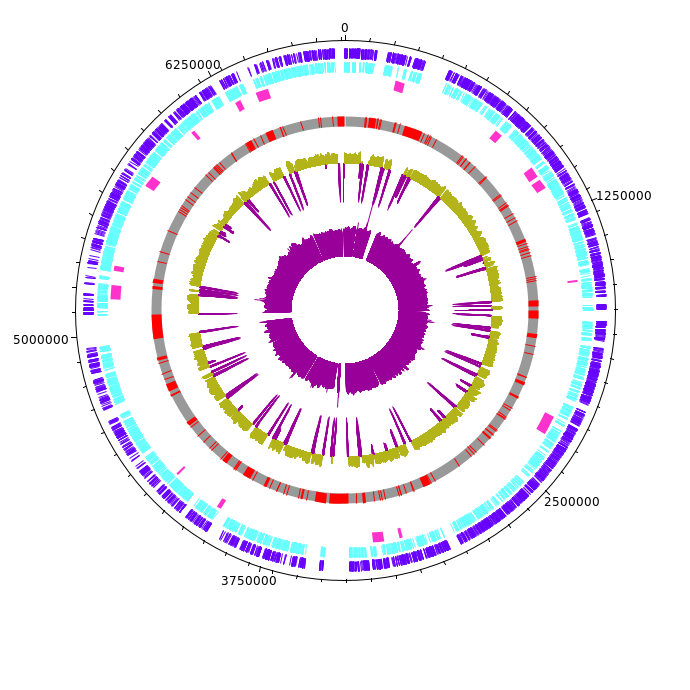
\includegraphics[width=0.8\linewidth]{imagens/genome/002.png} \\
	\centering
	\legend{Genes na direção \textit{foward} $($roxo$)$,
	Genes na direção \textit{reverse} $($azul claro$)$, \textit{clusters} gênicos $($rosa$)$,
	qualidade da montagem $($em cinza a montagem e em vermelho os \textit{gaps} da montagem$)$ e internamente 
	um gráfico representando a variação de conteúdo G$+$C $($amarelo quando maior que 50\% e roxo quando menor$)$ e
	mais internamente um gráfico representando o valor de G$+$C}
    \begin{small}\textbf{Fonte: autoria prória}\end{small}
\end{figure}
\vspace{\floatsep}

\begin{figure}[H]
	\caption{Gráficos representando a montagem do cromossomo da amostra 094}
	\label{fig:genoma94}
	\centering
	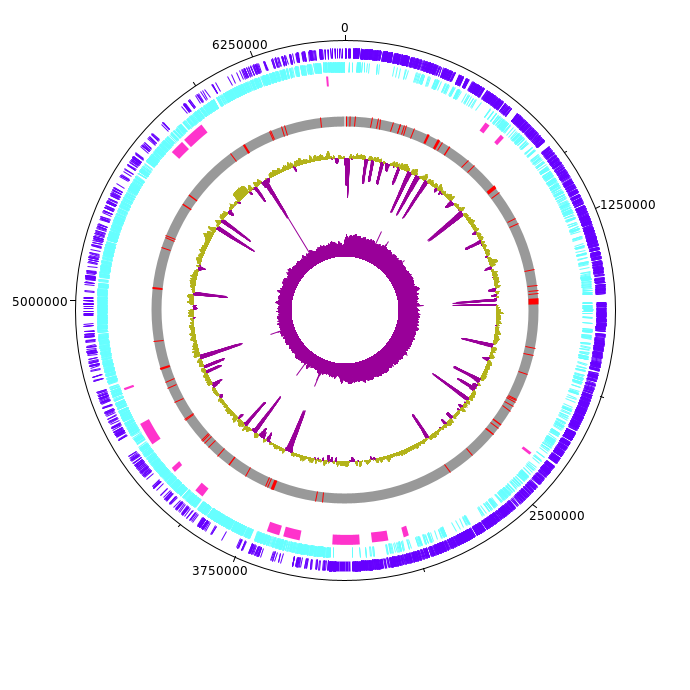
\includegraphics[width=0.8\linewidth]{imagens/genome/004.png} \\
	\centering
	\legend{Genes na direção \textit{foward} $($roxo$)$,
	Genes na direção \textit{reverse} $($azul claro$)$, \textit{clusters} gênicos $($rosa$)$,
	qualidade da montagem $($em cinza a montagem e em vermelho os \textit{gaps} da montagem$)$ e internamente 
	um gráfico representando a variação de conteúdo G$+$C $($amarelo quando maior que 50\% e roxo quando menor$)$ e
	mais internamente um gráfico representando o valor de G$+$C}
    \begin{small}\textbf{Fonte: autoria prória}\end{small}
\end{figure}
\vspace{\floatsep}


Através dessa visualização, podemos observar a sobreposição de alguns clusters gênicos com áreas
de \textit{gaps} na montagem, o que não desqualifica a predição desses clusters mas pode levar
a uma baixa identidades ou ausência de componentes nos clusters como genes acessórios importantes
para a síntese. O aprimoramento da montagem se faz necessário para o depósito desses genomas em 
bancos de dados de montagens. Esse pode ter sido um dos motivos para a baixa identificação dos
cluster na amostra 016.

\section{Predição de \textit{BGCs} e resistência a antimicrobianos}

Para a amostra 016, o software antishmash foi capaz de identificar 16 cluster biossintéticos completos, porém
apenas um cluster foi predito com 75\% de similaridade para produção de ectoína, um produto biosintético
conhecido e produzido por uma ampla gama de bactérias gram positivas e negativas \cite{stoveken2011specialized}.
Além disso, através da ferramenta armfinder foi observada a presença de genes codificando uma beta-lactamase de classe A e uma proteína de
proteção ribossomal ABC-F. A presença desses genes, pode indicar a resistência desse microrganismo a antibióticos beta-lactâmicos
e a macrolídeos.  

Já a amostra 094, teve 15 cluster biossintéticos preditos, dentro os quais 4 tiveram sua função identificada
por similaridade sendo produtores das seguintes substâncias e identidades percentuais: petrobactina$($83\%$)$, 
tyrocidina$($81\%$)$, gramicidina$($91\%$)$ e macrobrevina ($($100\%$)$). 


 \begin{figure}[H]
	\caption{\textit{Cluster biosintético} para produção de petrobactina na amostra 094}
	\label{fig:quast_16}
	\centering
		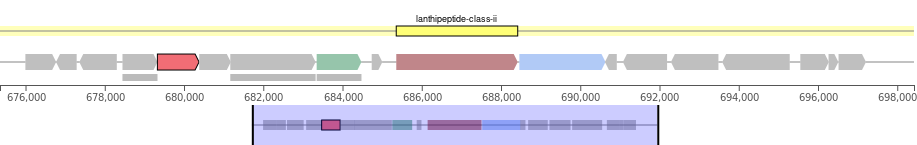
\includegraphics[width=0.8\linewidth]{imagens/antismash/094regiao1.png} \\
	\centering
    \begin{small}\textbf{Fonte: autoria prória}\end{small}
\end{figure}
\vspace{\floatsep}

A petrobactina é um sideróforo com protoreatividade capaz de reduzir ferro $III$ em 
ferro $II$\cite{barbeau2002petrobactin}. Interessantemente o cluster presente na amostra 94
capaz de produzir petrobactina, contém uma proteína de resistência tipo A a vancomicina e teicoplanina.

\begin{figure}[H]
	\caption{\textit{Cluster biosintético} para produção de tirocidina na amostra 094}
	\label{fig:quast_16}
	\centering
		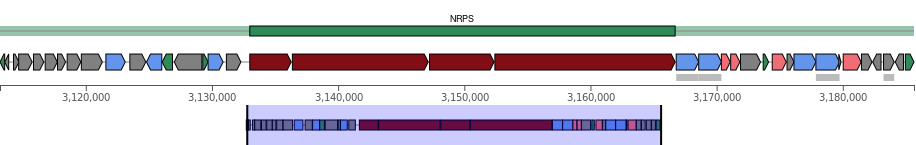
\includegraphics[width=0.8\linewidth]{imagens/antismash/094regiao2.png} \\
	\centering
    \begin{small}\textbf{Fonte: autoria prória}\end{small}
\end{figure}
\vspace{\floatsep}

\begin{figure}[H]
	\caption{\textit{Cluster biosintético} para produção de gramicidina na amostra 094}
	\label{fig:quast_16}
	\centering
		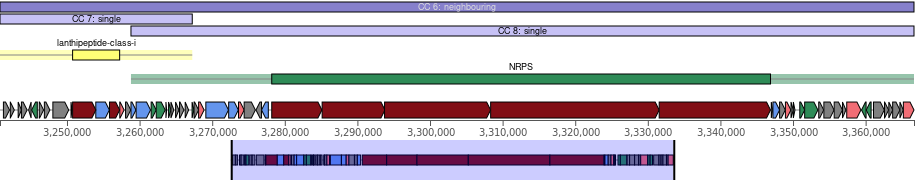
\includegraphics[width=0.8\linewidth]{imagens/antismash/094regiao3.png} \\
	\centering
    \begin{small}\textbf{Fonte: autoria prória}\end{small}
\end{figure}
\vspace{\floatsep}

A gramicidina e tirocidina são peptídeos lineares de síntese não ribossomal, com mecanismo de ação
através do dano na membrana celular de outros organismos, a tirocidina é relatada como um candidato importante
a antibiótico de nova geração por não ter induzido resistência nas células afetadas\cite{yang2018antimicrobial}.
A presença de clusters capazes de produzir não apenas um mas dois tipos diferentes de peptídeos com
atividade antimicrobiana sugere atividade antimicrobiana no isolado 094, o que precisa ser elucidado através
de testes \textit{in vitro} em condições que promovam a expressão desses compostos para posterior purificação e
descrição de suas estruturas através da técnica de espectometria de massa.

\begin{figure}[H]
	\caption{\textit{Cluster biosintético} para produção de macrobrevina na amostra 094}
	\label{fig:quast_16}
	\centering
		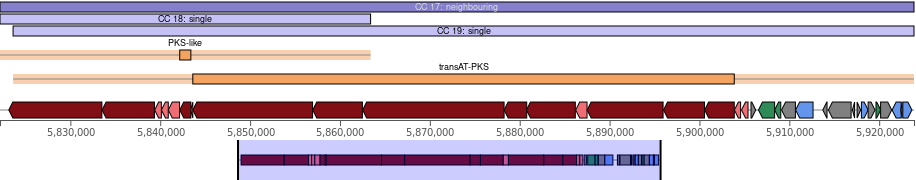
\includegraphics[width=0.8\linewidth]{imagens/antismash/094regiao4.png} \\
	\centering
    \begin{small}\textbf{Fonte: autoria prória}\end{small}
\end{figure}
\vspace{\floatsep}

O cluster de produção para macrobrevina foi o único encontrado com 100\% de similaridade na amostra
094, esse antibiótico com estrutura incomum derivado de uma trans-aciltransferase policetídeo sintase foi inicialmente isolado
a partir de \textit{Brevibacillus sp.} associados ao microbioma de plantas \cite{helfrich2018bipartite}.

A amostra 016 apresenta diversos \textit{cluster} e através de métodos computacionais utilizando bancos
de dados extensos não fomos capazes de predizer a função desses clusters, o que ressalta a importância de 
estudos de purificação e descrição das estruturas desses compostos.

Diferentemente, a amostra 094 apresenta 3 clusters identificados como produtores de produtos naturais com
ativade antimicrobiana, o que deve ser confirmado através de ensaios elaborados que promovam a expressão
desses genes e para sua posterior purificação. Esse microrganismo tem grande potêncial para descrição de 
produtos naturais com atividade antimicrobiana, apesar de serem de classes conhecidas. A elucidação dessas
estruturas pode sugerir modificações em antibióticos derivados dessa substância, e também ajudar a complementar
informações já existentes a respeito da produção de compostos de interesse biotecnológicos em \textit{Brevibacillus brevis}.

Quanto a presença de genes de resistência a amostra 94 teve a resistência predita para antibióticos como clorofenicol,
Kanamicinda, Tobramicina, streptomicina, lincossamida, macrolídeos, streptogramina, macrolídeos e beta-lactâmicos. 

	\begin{table}[htb]
		\IBGEtab{%
		  \caption{Informações a respeito dos alinhamentos para predição de \textit{ARGs}}%
		  \label{tabela-args}
		}{%
		\begin{tabular}{ccccc}
		 \toprule
		 \textbf{CDS da \textit{query}} & \textbf{Abrev. do Gene} & \textbf{Cobertura $($\%$)$} & \textbf{ Identidade $($\%$)$} & \textbf{Comprimento} \\
		  \midrule 
		  004\_01565                                    & catV                                          & 100.00                                                    & 94.52                                                      & 219                                                             \\
		  004\_04575                                    & ant(4')-Ic                                    & 100.00                                                    & 93.36                                                      & 256                                                             \\
		  004\_02000                                    & aac(6')-35                                    & 100.00                                                    & 92.74                                                      & 179                                                             \\
		  004\_02604                                    & ant(6)-Ic                                     & 100.00                                                    & 91.61                                                      & 286                                                             \\
		  004\_02904                                    & clbC                                          & 100.00                                                    & 90.96                                                      & 343                                                             \\
		  004\_00361                                    & mphJ                                          & 99.68                                                     & 88.60                                                      & 307                                                             \\
		  004\_01265                                    & blaBBI                                        & 100.00                                                    & 87.83                                                      & 304                                                             \\
		  \bottomrule
		\end{tabular}
		}{%
		 \centering
		  \fonte{ autoria prória}%
		  \legend{Informações obtidas a partir dos alinhamentos de sequência realizados pela
		  ferramenta armfinder}%
		  }
		\end{table}

Os alinhamentos demonstram a presença de vários genes relacionados a resistência, inclusive a classes inteiras de antibióticos 
como beta-lactâmicos e macrolídeos, devido ao grande espectro de proteção conferidos por esses genes. 
